\documentclass[multi=tikzpicture,border=7pt]{standalone}
\usepackage{ctex,amsmath,bm}
\usepackage{tikz,pgfplots}
\pgfplotsset{compat=1.18}
\usetikzlibrary{arrows.meta,calc,angles,quotes,patterns,positioning,decorations.pathmorphing,3d}
\tikzset{wire/.style={brown!70!black,very thick},guide/.style={dashed,gray!60},force/.style={->,>=Stealth,thick,red!70!black},velocity/.style={->,>=Stealth,thick,blue!70!black},axis/.style={->,>=Stealth,thick},dim/.style={<->,>=Stealth,thin},body/.style={draw,thick,fill=blue!7},panel/.style={anchor=west,font=\bfseries},hidden/.style={dashed,gray!58,thick},orbit/.style={very thick,blue!70!black}}
\tikzset{vec/.style={->,>=Stealth,very thick},wall/.style={pattern=north east lines,pattern color=gray},nodept/.style={circle,fill=white,draw,inner sep=1.5pt}}
\begin{document}
% 1 question-01
\begin{tikzpicture}[x=1cm,y=1cm,font=\small]

\draw[body](0,0)circle(1.8);\fill(0,-1.8)circle(2pt)node[below]{$O$};\draw[velocity](0,-1.8)--(-1.3,-1.8)node[left]{$av_0$};\draw[force](0,-1.8)--(1.3,-1.8)node[right]{$bv_0$};\draw[dim](0,-1.4)arc[start angle=270,end angle=330,radius=1.4];\node at(1.5,-1){$x$};\node at(0,2.4){逆时针为位置正向，$t=0$ 不计碰撞};
\end{tikzpicture}

% 2 solution-01
\begin{tikzpicture}[x=1cm,y=1cm,font=\small]

\draw[axis](0,0)--(5,0)node[right]{$\tau=(a+b)v_0t/L$};\draw[axis](0,-2.2)--(0,2.9)node[above]{$s/L$};
\foreach\k in{-1,0,1,2}{\draw[velocity](0,\k)--(4,{\k-4*3/14});}
\draw[force](0,0)--(4,{4*11/14});
\foreach\k in{1,2,3}{\fill(\k,{11*\k/14})circle(1.8pt);\draw[guide](\k,0)--(\k,{11*\k/14});\node[below]at(\k,0){$\k$};}
\node[right]at(3.3,2.65){$s_B=11\tau/14$};\node[right]at(3.5,-1.5){$s_A=-3\tau/14+n$};
\node at(2,-2.8){交点纵坐标取模：$x_k/L=\{11k/14\}$，共14点};
\end{tikzpicture}

% 3 question-02
\begin{tikzpicture}[x=1cm,y=1cm,font=\small]
\begin{scope}[shift={(-3.6,1.8)}]
\node[above]at(1,1.75){选项A};
\draw[wire](0,1)--(2,1)node[midway,fill=white,draw,inner sep=3pt]{$ C $};
\draw[wire](0,1)--(2,-1)node[midway,fill=white,draw,inner sep=3pt]{$ L $};
\draw[wire](2,1)--(2,-1)node[midway,fill=white,draw,inner sep=3pt]{$ R $};
\fill(0,1)circle(1.6pt)node[left]{$1$};\fill(2,1)circle(1.6pt)node[right]{$3$};\fill(2,-1)circle(1.6pt)node[right]{$2$};
\end{scope}
\begin{scope}[shift={(1.1999999999999997,1.8)}]
\node[above]at(1,1.75){选项B};
\draw[wire](0,1)--(1,1)node[midway,fill=white,draw,inner sep=3pt]{$ L $};
\draw[wire](1,1)--(2,1)node[midway,fill=white,draw,inner sep=3pt]{$ R $};
\draw[wire](1,1)--(1,-1)node[midway,fill=white,draw,inner sep=3pt]{$ C $};
\fill(0,1)circle(1.6pt)node[left]{$1$};\fill(2,1)circle(1.6pt)node[right]{$3$};\fill(2,-1)circle(1.6pt)node[right]{$2$};
\draw[wire](1,-1)--(2,-1);\end{scope}
\begin{scope}[shift={(-3.6,-1.9999999999999998)}]
\node[above]at(1,1.75){选项C};
\draw[wire](0,1)--(1,1)node[midway,fill=white,draw,inner sep=3pt]{$ C $};
\draw[wire](1,1)--(2,1)node[midway,fill=white,draw,inner sep=3pt]{$ L $};
\draw[wire](2,1)--(2,-1)node[midway,fill=white,draw,inner sep=3pt]{$ R $};
\fill(0,1)circle(1.6pt)node[left]{$1$};\fill(2,1)circle(1.6pt)node[right]{$3$};\fill(2,-1)circle(1.6pt)node[right]{$2$};
\end{scope}
\begin{scope}[shift={(1.1999999999999997,-1.9999999999999998)}]
\node[above]at(1,1.75){选项D};
\draw[wire](0,1)--(1,1)node[midway,fill=white,draw,inner sep=3pt]{$ L $};
\draw[wire](1,1)--(2,1)node[midway,fill=white,draw,inner sep=3pt]{$ R $};
\draw[wire](2,1)--(2,-1)node[midway,fill=white,draw,inner sep=3pt]{$ C $};
\fill(0,1)circle(1.6pt)node[left]{$1$};\fill(2,1)circle(1.6pt)node[right]{$3$};\fill(2,-1)circle(1.6pt)node[right]{$2$};
\end{scope}
\node at(0,-4.1){电源接1、2；表接3、2，理想A短路、V开路};
\end{tikzpicture}

% 4 solution-02
\begin{tikzpicture}[x=1cm,y=1cm,font=\small]

\begin{scope}[shift={(-3.5,0)}]\draw[wire](-1,1)--(0,1)node[midway,fill=white,draw]{$L$};\draw[wire](0,1)--(1,1)node[midway,fill=white,draw]{$R$};\draw[wire](1,1)--(1,-1)node[midway,fill=white,draw]{$C$};\draw[guide](1,1)--(2,1)--(2,-1)--(1,-1);\node[right]at(2,0){A/V};\fill(-1,1)circle(1.5pt)node[left]{$1$};\fill(1,1)circle(1.5pt)node[above]{$3$};\fill(1,-1)circle(1.5pt)node[below]{$2$};\node at(.5,-2){D：$1-L-R-3-C-2$};\end{scope}
\begin{scope}[shift={(3.5,0)}]\draw[axis](-.3,0)--(2.5,0)node[right]{$\Re Z/R$};\draw[axis](0,-2.2)--(0,1.5)node[above]{$\Im Z/R$};\draw[velocity](0,0)--(1,.57735)node[right]{$Z_A/R$};\draw[force](0,0)--(1,-1.73205)node[right]{$Z_V/R$};\draw[guide](1,.57735)--(1,-1.73205);\node at(1.7,1.2){$+30^\circ$};\node at(1.85,-1){$-60^\circ$};\node at(.5,-2.8){电容电压相对电流 $-90^\circ$};\end{scope}
\end{tikzpicture}

% 5 question-03
\begin{tikzpicture}[x=1cm,y=1cm,font=\small]

\draw[thick](0,-1.6)--(0,3.6);\fill(0,2.4)circle(2pt)node[left]{$O$};\draw[wire](0,2.4)--(-1.5,.7)--(0,-1)--(1.5,.7)--cycle;
\draw[body](-1.5,.7)circle(.14)node[left]{$m$};\draw[body](1.5,.7)circle(.14)node[right]{$m$};\draw[body](-.28,-1.2)rectangle(.28,-.8);\node[left]at(-.4,-1){$M$};\node[left]at(-.9,1.7){$l$};\node[left]at(-.9,-.3){$l$};\draw[dim](2.4,-1)--(2.4,2.4)node[right,midway]{$h$};\draw[velocity](.45,3.3)arc[start angle=30,end angle=300,radius=.4];\node[right]at(.85,3.2){$\omega$};\node at(.4,-2){四杆等长，套筒随轴转动；几何位置示意};
\end{tikzpicture}

% 6 solution-03
\begin{tikzpicture}[x=1cm,y=1cm,font=\small]
\draw[axis](0,0)--(3.45,0)node[right]{$\omega/(\mathrm{rad\,s^{-1}})$};\draw[axis](0,0)--(0,4.25)node[above]{$P/\mathrm{kW}$};\draw[velocity]plot[smooth]coordinates{(0.00000,0.01418) (0.02800,0.04335) (0.05600,0.07251) (0.08400,0.10167) (0.11200,0.13081) (0.14000,0.15994) (0.16800,0.18906) (0.19600,0.21817) (0.22400,0.24727) (0.25200,0.27636) (0.28000,0.30544) (0.30800,0.33452) (0.33600,0.36358) (0.36400,0.39263) (0.39200,0.42167) (0.42000,0.45071) (0.44800,0.47973) (0.47600,0.50874) (0.50400,0.53775) (0.53200,0.56674) (0.56000,0.59573) (0.58800,0.62470) (0.61600,0.65367) (0.64400,0.68263) (0.67200,0.71157) (0.70000,0.74051) (0.72800,0.76944) (0.75600,0.79836) (0.78400,0.82727) (0.81200,0.85617) (0.84000,0.88506) (0.86800,0.91394) (0.89600,0.94281) (0.92400,0.97167) (0.95200,1.00052) (0.98000,1.02937) (1.00800,1.05820) (1.03600,1.08703) (1.06400,1.11584) (1.09200,1.14465) (1.12000,1.17345) (1.14800,1.20224) (1.17600,1.23102) (1.20400,1.25979) (1.23200,1.28855) (1.26000,1.31730) (1.28800,1.34604) (1.31600,1.37478) (1.34400,1.40350) (1.37200,1.43222) (1.40000,1.46092) (1.42800,1.48962) (1.45600,1.51831) (1.48400,1.54699) (1.51200,1.57566) (1.54000,1.60432) (1.56800,1.63298) (1.59600,1.66162) (1.62400,1.69026) (1.65200,1.71888) (1.68000,1.74750) (1.70800,1.77611) (1.73600,1.80471) (1.76400,1.83330) (1.79200,1.86189) (1.82000,1.89046) (1.84800,1.91903) (1.87600,1.94758) (1.90400,1.97613) (1.93200,2.00467) (1.96000,2.03320) (1.98800,2.06172) (2.01600,2.09024) (2.04400,2.11874) (2.07200,2.14724) (2.10000,2.17573) (2.12800,2.20421) (2.15600,2.23268) (2.18400,2.26114) (2.21200,2.28959) (2.24000,2.31804) (2.26800,2.34648) (2.29600,2.37491) (2.32400,2.40333) (2.35200,2.43174) (2.38000,2.46014) (2.40800,2.48854) (2.43600,2.51692) (2.46400,2.54530) (2.49200,2.57367) (2.52000,2.60203) (2.54800,2.63039) (2.57600,2.65873) (2.60400,2.68707) (2.63200,2.71540) (2.66000,2.74372) (2.68800,2.77203) (2.71600,2.80034) (2.74400,2.82864) (2.77200,2.85692) (2.80000,2.88520)};\draw[force]plot[smooth]coordinates{(0.00000,1.01326) (0.02800,1.01257) (0.05600,1.01188) (0.08400,1.01119) (0.11200,1.01050) (0.14000,1.00981) (0.16800,1.00912) (0.19600,1.00844) (0.22400,1.00775) (0.25200,1.00706) (0.28000,1.00638) (0.30800,1.00569) (0.33600,1.00501) (0.36400,1.00433) (0.39200,1.00364) (0.42000,1.00296) (0.44800,1.00228) (0.47600,1.00160) (0.50400,1.00092) (0.53200,1.00024) (0.56000,0.99956) (0.58800,0.99889) (0.61600,0.99821) (0.64400,0.99753) (0.67200,0.99686) (0.70000,0.99618) (0.72800,0.99551) (0.75600,0.99484) (0.78400,0.99416) (0.81200,0.99349) (0.84000,0.99282) (0.86800,0.99215) (0.89600,0.99148) (0.92400,0.99081) (0.95200,0.99014) (0.98000,0.98947) (1.00800,0.98880) (1.03600,0.98814) (1.06400,0.98747) (1.09200,0.98681) (1.12000,0.98614) (1.14800,0.98548) (1.17600,0.98481) (1.20400,0.98415) (1.23200,0.98349) (1.26000,0.98283) (1.28800,0.98217) (1.31600,0.98151) (1.34400,0.98085) (1.37200,0.98019) (1.40000,0.97953) (1.42800,0.97887) (1.45600,0.97822) (1.48400,0.97756) (1.51200,0.97691) (1.54000,0.97625) (1.56800,0.97560) (1.59600,0.97494) (1.62400,0.97429) (1.65200,0.97364) (1.68000,0.97299) (1.70800,0.97234) (1.73600,0.97169) (1.76400,0.97104) (1.79200,0.97039) (1.82000,0.96974) (1.84800,0.96909) (1.87600,0.96844) (1.90400,0.96780) (1.93200,0.96715) (1.96000,0.96651) (1.98800,0.96586) (2.01600,0.96522) (2.04400,0.96458) (2.07200,0.96393) (2.10000,0.96329) (2.12800,0.96265) (2.15600,0.96201) (2.18400,0.96137) (2.21200,0.96073) (2.24000,0.96009) (2.26800,0.95946) (2.29600,0.95882) (2.32400,0.95818) (2.35200,0.95755) (2.38000,0.95691) (2.40800,0.95628) (2.43600,0.95564) (2.46400,0.95501) (2.49200,0.95437) (2.52000,0.95374) (2.54800,0.95311) (2.57600,0.95248) (2.60400,0.95185) (2.63200,0.95122) (2.66000,0.95059) (2.68800,0.94996) (2.71600,0.94933) (2.74400,0.94871) (2.77200,0.94808) (2.80000,0.94745)};\fill(0.9421496437842691,0.9903747149857759)circle(1.8pt);\draw[guide](0.9421496437842691,0)--(0.9421496437842691,0.9903747149857759);\node[below]at(0,0){$2.05$};\node[below]at(2.8,0){$2.12$};\node[below]at(0.9421496437842691,0){$2.074$};\node[left]at(0,1){$2.5$};\node[right]at(2.7,2.9){$P_d$};\node[right]at(2.7,.7){$P_{\rm motor}$};\node at(1.6,-.9){交点为准静态工作点；高速侧负功率差};
\end{tikzpicture}

% 7 question-04
\begin{tikzpicture}[x=1cm,y=1cm,font=\small]

\draw[axis](-4,0)--(5.5,0);\draw[body,fill=none](0,0)ellipse[x radius=.22,y radius=1.2];\draw[thick](4.2,-1.2)--(4.2,1.2)node[above]{视网膜};\fill(-3,.8)circle(1.8pt)node[above]{$P$};
\draw[velocity](-3,.8)--(0,1)--(4,-.2)--(5,-.5);\draw[velocity](-3,.8)--(0,-1)--(4,-.2)--(5,0);\draw[guide](4,-1)--(4,.8);\node[below left]at(4,-.65){几何像};\draw[guide](4,-.6)--(4,-.2);\draw[dim](-.7,-1)--(-.7,1)node[left,midway]{$D$};\draw[dim](0,-1.7)--(4.2,-1.7)node[below,midway]{$d$};\node at(.5,-2.3){此物距下近视眼焦点在视网膜前；视网膜截取光锥为弥散斑};
\end{tikzpicture}

% 8 solution-04
\begin{tikzpicture}[x=1cm,y=1cm,font=\small]

\draw[axis](-.5,0)--(5.5,0);\draw[body,fill=none](0,0)ellipse[x radius=.2,y radius=1.2];\draw[thick](4.2,-1.2)--(4.2,1.2);\draw[guide](4,-.8)--(4,.8);
\draw[velocity](0,1)--(4,.3)--(5,.125);\draw[velocity](0,-1)--(4,.3)--(5,.625);\fill(4,.3)circle(1.5pt);\draw[guide](4,.3)--(3.3,1.15);\node[above left]at(3.3,1.15){几何焦点};\draw[force](4.2,.265)--(4.2,.365);\draw[guide](4.2,.315)--(5.1,.85);\node[right]at(5.1,.85){$2r_b$};\node[above]at(4.2,1.5){视网膜};\draw[dim](0,-1.7)--(4.2,-1.7)node[below,midway]{$d$};\draw[dim](4,-1.1)--(4.2,-1.1);\draw[guide](4.1,-1.1)--(5,-1.65);\node[right]at(5,-1.65){$d-v$};\node at(2.5,-2.45){$r_b=(D/2)(d/v-1)$；物方距离由 $u/d$ 反算};
\end{tikzpicture}

% 9 question-05
\begin{tikzpicture}[x=1cm,y=1cm,font=\small]
\coordinate(N0)at(0.00000,2.00000);\fill(N0)circle(2pt)node[shift={(0.000,0.350)}]{$ 0 $};
\coordinate(N1)at(1.73205,1.00000);\fill(N1)circle(2pt)node[shift={(0.303,0.175)}]{$ 1 $};
\coordinate(N2)at(1.73205,-1.00000);\fill(N2)circle(2pt)node[shift={(0.303,-0.175)}]{$ 2 $};
\coordinate(N3)at(0.00000,-2.00000);\fill(N3)circle(2pt)node[shift={(0.000,-0.350)}]{$ 3 $};
\coordinate(N4)at(-1.73205,-1.00000);\fill(N4)circle(2pt)node[shift={(-0.303,-0.175)}]{$ 4 $};
\coordinate(N5)at(-1.73205,1.00000);\fill(N5)circle(2pt)node[shift={(-0.303,0.175)}]{$ 5 $};
\draw[velocity,-](N0)--(N1)node[midway,fill=white,draw]{$C$};
\draw[velocity,-](N1)--(N2)node[midway,fill=white,draw]{$C$};
\draw[velocity,-](N2)--(N3)node[midway,fill=white,draw]{$C$};
\draw[velocity,-](N3)--(N4)node[midway,fill=white,draw]{$C$};
\draw[velocity,-](N4)--(N5)node[midway,fill=white,draw]{$C$};
\draw[velocity,-](N5)--(N0)node[midway,fill=white,draw]{$C$};
\draw[wire,decorate,decoration={coil,aspect=.5,segment length=5pt,amplitude=2pt}](N0)--(N2);
\draw[wire,decorate,decoration={coil,aspect=.5,segment length=5pt,amplitude=2pt}](N1)--(N3);
\draw[wire,decorate,decoration={coil,aspect=.5,segment length=5pt,amplitude=2pt}](N2)--(N4);
\draw[wire,decorate,decoration={coil,aspect=.5,segment length=5pt,amplitude=2pt}](N3)--(N5);
\draw[wire,decorate,decoration={coil,aspect=.5,segment length=5pt,amplitude=2pt}](N4)--(N0);
\draw[wire,decorate,decoration={coil,aspect=.5,segment length=5pt,amplitude=2pt}](N5)--(N1);
\node at(0,-2.9){蓝色：相邻电容；棕色：次近邻电感，交叉不相通};
\end{tikzpicture}

% 10 solution-05
\begin{tikzpicture}[x=1cm,y=1cm,font=\small]

\draw[axis](-.6,0)--(6,0)node[right]{$m$};\draw[axis](0,-.4)--(0,3.8)node[above]{$\omega^2LC$};\foreach\x/\y in{1/3,2/1,3/0,4/1,5/3}{\draw[velocity,-](\x,0)--(\x,\y);\fill[blue!70!black](\x,\y)circle(2pt);\node[below]at(\x,0){$\x$};}\node[below]at(0,0){$0$};\node[left]at(0,1){$1$};\node[left]at(0,3){$3$};\node[above]at(2.9,3.3){$m=1,5$ 简并；$m=2,4$ 简并};\node at(3,-1){$m=0$：等势规范，无频率；$m=3$：静态零模};
\end{tikzpicture}

% 11 question-06
\begin{tikzpicture}[x=1cm,y=1cm,font=\small]
\coordinate(O)at(0,0);\coordinate(A)at(0,.8);\coordinate(B)at(1.2,2.87846);\coordinate(C)at(2.4,.8);\draw[thick](-.5,0)--(3,0);\draw[wire](O)--(A)--(B)--(C);\draw[guide](2.4,.2)--(2.4,3.2);\draw[body](2.24,.62)rectangle(2.56,.98);\foreach\p in{O,A,B,C}{\fill(\p)circle(1.8pt)node[above right]{$\p$};}\node[left]at(0,.35){$l$};\node[left]at(.6,1.8){$3l$};\node[right]at(1.8,1.8){$3l$};\node at(1.3,-.6){$AB,BC$ 与竖直夹角 $30^\circ$};\draw[velocity](A)--(-1,.8)node[left]{$\omega l$};\draw[velocity](C)--(2.4,1.9)node[right]{$v_0$};
\end{tikzpicture}

% 12 solution-06
\begin{tikzpicture}[x=1cm,y=1cm,font=\small]
\coordinate(O)at(0,0);\coordinate(A)at(0,.8);\coordinate(B)at(1.2,2.87846);\coordinate(C)at(2.4,.8);\draw[thick](-.5,0)--(3,0);\draw[wire](O)--(A)--(B)--(C);\draw[guide](2.4,.2)--(2.4,3.2);\draw[body](2.24,.62)rectangle(2.56,.98);\foreach\p in{O,A,B,C}{\fill(\p)circle(1.8pt)node[above right]{$\p$};}\node[left]at(0,.35){$l$};\node[left]at(.6,1.8){$3l$};\node[right]at(1.8,1.8){$3l$};\node at(1.3,-.6){$AB,BC$ 与竖直夹角 $30^\circ$};\draw[velocity](A)--(-1,.8)node[left]{$\bm v_A$};\draw[velocity](C)--(2.4,1.9)node[right]{$\bm v_C$};\draw[velocity](B)--(-.16,3.09)node[left]{$\bm v_B$};\draw[force](B)--(1.104,1.86)node[left]{$\bm a_B$};\draw[force](A)--(0,-.25)node[left]{$\bm a_A$};\node at(1.3,-1.2){$B$ 箭头示例：$\omega l=v_0$、$a_0=0$};
\end{tikzpicture}

% 13 question-07
\begin{tikzpicture}[x=1cm,y=1cm,font=\small]
\draw[thick](-2,0)--(4,0);\draw[body](0,.7)circle(.7);\draw[body](.7,1.91244)circle(.7);\draw[body](1.4,.7)circle(.7);\node at(0,.7){$A$};\node at(.7,1.91244){$B$};\node at(1.4,.7){$C$};\draw[guide](0,.7)--(.7,1.91244)--(1.4,.7);\node[left]at(0,1.6){$2R$};\node[right]at(1.5,1.6){$2R$};\node at(1,-.65){$A$ 固定，$B:m$、$C:nm$；初始 $\theta=60^\circ$};
\end{tikzpicture}

% 14 solution-07
\begin{tikzpicture}[x=1cm,y=1cm,font=\small]

\draw[thick](-1.5,0)--(4.5,0);\coordinate(A)at(0,.7);\coordinate(B)at(.94376,1.73399);\coordinate(C)at(1.88752,.7);\foreach\p in{A,B,C}{\draw[body](\p)circle(.7);\node at(\p){$\p$};}\draw[guide](A)--(B)--(C);\draw[velocity](B)--++(.7,-.64)node[right]{$\bm v_B$};\draw[velocity](C)--++(1,0)node[below]{$\bm v_C$};\draw[force](B)--++(.54,.59)node[above]{$N_{AB}$};\draw[force](B)--++(-.54,.59)node[left]{$N_{BC}$};\draw[force](B)--++(0,-.85)node[left]{$mg$};
\draw[velocity](1.494,2.304)arc[start angle=46,end angle=-30,radius=.8];\node[right]at(1.7,2.45){$\omega_B<0$};\draw[velocity](2.58,.3)arc[start angle=-30,end angle=46,radius=.8];\node[right]at(2.8,1.25){$\omega_C>0$};\node at(1.3,-.8){有限摩擦先失去无滑动；第6问缺摩擦与惯量条件};
\end{tikzpicture}

% 15 question-08
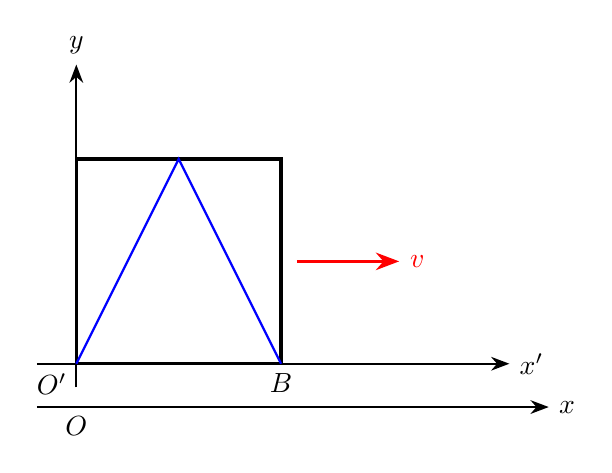
\begin{tikzpicture}
  \draw[axis] (-.5,0)--(5.5,0) node[right]{$x'$}; \draw[axis] (0,-.3)--(0,3.8) node[above]{$y$};
  \draw[very thick] (0,0) rectangle(2.6,2.6); \node[below left] at (0,0){$O'$}; \node[below] at (2.6,0){$B$};
  \draw[blue,thick] (0,0)--(1.3,2.6)--(2.6,0); \draw[vec,red] (2.8,1.3)--++(1.3,0) node[right]{$v$};
  \draw[axis] (-.5,-.55)--(6,-.55) node[right]{$x$}; \node[below] at (0,-.55){$O$};
\end{tikzpicture}

% 16 solution-08
\begin{tikzpicture}[x=1cm,y=1cm,font=\small]
\begin{scope}[shift={(-3,0)}]\draw[body](0,0)rectangle(2,2);\fill(0,0)circle(1.6pt)node[below]{$O^{\prime}$};\fill(1,2)circle(1.6pt)node[above]{$M$};\fill(2,0)circle(1.6pt)node[below]{$B$};\draw[velocity](0,0)--(1,2)--(2,0);\node at(1,-.8){车厢系光路；$t_B^{\prime}=\sqrt5l/c$};\end{scope}
\begin{scope}[shift={(1.5,0)}]\draw[axis](-.4,0)--(3.5,0)node[right]{$x/l$};\draw[axis](0,-.3)--(0,3.5)node[above]{$ct/l$};\draw[guide](0,0)--(1.2800000000000002,3.2);\draw[guide](0.9165151389911681,0)--(2.1965151389911686,3.2);\draw[velocity](0,0)--(1.0334947620642474,1.4380929814216588)--(2.066989524128495,2.8761859628433175);\fill(1.0334947620642474,1.4380929814216588)circle(1.8pt)node[left]{$E_M$};\fill(2.066989524128495,2.8761859628433175)circle(1.8pt)node[right]{$E_B$};\draw[guide](0.45825756949558405,0)--(1.7382575694955844,3.2);\draw[dashed,orange!80!black](0,2.8761859628433175)--(2.066989524128495,2.8761859628433175);\draw[dash dot,green!50!black](0,2.0493901531919194)--(2.8,3.1693901531919195);\node[above]at(1.2800000000000002,3.2){$O^{\prime}$};\node[above]at(1.7382575694955844,3.2){$M$};\node[above]at(2.1965151389911686,3.2){$B$};\node at(1.6,-.8){$\beta=0.4$；橙：地面同时，绿：车厢同时};\node at(1.6,-1.4){$x$—$ct$ 是光路投影；竖直轴为地面 $O$ 世界线};\end{scope}
\end{tikzpicture}

\end{document}
